\chapter{Security in Earnest II \small{\textsf{DRAFT}}}\label{chapter:earnest2}
\section{Safety and Liveness}

\subsection{Defining Safety and Liveness}
Now that we have formally defined the synchronous model underlying our blockchain (in the previous lecture), we now rigorously define the security properties that a blockchain-based ledger must satisfy, notably, \textit{safety} and \textit{liveness}.

% Blockchains achieve safety when all honest parties have views of the ledgers that are all prefixes of one another. More specifically, one party's view of the ledger at some previous round must be a prefix of the view of another party's ledger at a later round. Blockchains achieve liveness if when an honest party submits a transaction at round $r$, then the transaction is in the ledgers of all other honest parties by round $r + u$. We formalize these definitions as follows.
% Denote by $L^P_r$ the ledger of party $P$ at round $r$.

A ledger achieves safety when all honest parties have views of the ledger that are consistent with one another. More precisely, any transaction included in one party's ledger at a specific round is also included at the same position in all other parties' ledgers at all later rounds.
A ledger achieves liveness if whenever honest parties attempt to add a transaction to the ledger, it gets added to all parties' ledgers within $u$ rounds.

\begin{itemize}
\item \textbf{Safety:} For all honest parties $P_1, P_2$, and rounds $r_1 < r_2$,
$\forall i \in [|L_{r_1}^{P_1}|]$,
a transaction reported at
$L^{P_1}_{r_1}[i]$ also appears at $L^{P_2}_{r_2}[i]$.

\item \textbf{Liveness($u$)}: If all honest parties attempt to inject a transaction $\mathsf{tx}$ at rounds $r,...,r+u$, then for all honest parties $P$, $\mathsf{tx}$ will appear in $L_{r+u}^P$.
\end{itemize}

Note that $u$ should be defined so that it is at least large enough that an honest party successfully creates and broadcasts a block in $u$ rounds, and that block gets buried under $k$ blocks.

Now that safety and liveness are defined, we will prove how satisfying the chain virtues common prefix, chain quality, and chain growth implies that safety and liveness hold.

\subsection{Common Prefix Implies Safety}

\begin{theorem} If the longest chain protocol satisfies $CP(k)$, then the resulting ledger is safe.
\end{theorem}

\begin{proof}
    Let $C_1$ be the view of party $P_1$ at round $r_1$, and $C_2$ be the view of $P_2$ at round $r_2$; where $r_1 < r_2$. Because $CP(k)$ is satisfied, the condition $C_1[:-k] \preceq C_2$ must hold. The honest protocol states that for a transaction $\mathsf{tx}$ to appear in the ledger of an honest party, $\mathsf{tx}$ must be buried under $k$ blocks in the honest party's chain. Therefore, we know that $L^{P_1}_{r_1}$ is made up of the transactions in $C_1[:-k]$, because $C_1[:-k]$ is buried $k$ blocks deep from the longest chain tip.
    We know that $C_1[:-k] \preceq C_2$ due to common prefix. Moreover, each block in $C_1[:-k]$ must be buried at least $k$ blocks deep in $C_2$ because the honest node $P_1$ must have broadcast $C_1$ in or before round $r_1$ and due to the longest chain rule, $|C_2| \geq |C_1|$. Hence, $L^{P_1}_{r_1}$ is a prefix of $L^{P_2}_{r_2}$. This implies that all transactions in $L^{P_1}_{r_1}$ must also be included in $L^{P_2}_{r_2}$ at the same positions, and hence safety holds.
\end{proof}

% \begin{center}
% \begin{tikzpicture}

% % Sum shape

% % Controller
% \node [draw,
%     minimum width=0.5cm,
%     minimum height=0.5cm
% ]  (controller) {$G$};

% % System H(s)
% \node [draw,
%     minimum width=0.5cm,
%     minimum height=0.5cm,
%     right=1.5cm of controller
% ] (system) {$r - k$};

% % System H(s)
% \node [draw,
%     minimum width=0.5cm,
%     minimum height=0.5cm,
%     right=1.5cm of system
% ] (system2) {$r$};

% \draw[-stealth] (controller.east) -- (system.west)
%     node[midway,above]{$...$};

% \draw[-stealth] (system.east) -- (system2.west)
%     node[midway,above]{$k$};

% \end{tikzpicture}
% \end{center}

\subsection{Chain Quality and Chain Growth Imply Liveness}

\begin{theorem} If the protocol satisfies $CQ(\mu, \ell)$ and $CG(\tau,s)$ then the ledger satisfies liveness with $u = \max(\frac{\ell + k}{\tau}, s)$.
\end{theorem}

\begin{proof}
Due to the Chain Quality assumption CQ($\mu,\ell$), at least one block out of $\ell$ consecutive blocks in a chain will be honestly mined if $\mu \ell \geq 1$. Moreover, we require that for a block to be included in a ledger, it must be buried under $k$ blocks. Therefore, we know that an honestly mined block is included in the ledger if we wait for the honestly adopted chains to grow by $\ell + k$ blocks. Because $u\tau$ is the minimum growth of the honestly adopted chains in $u$ rounds, therefore, if we want liveness to hold with $u$, then we require that $u\tau \geq \ell+k$. However, in order to invoke Chain Growth at all, we need to wait at least $s$ rounds, therefore, the above only holds if $u \geq s$ also holds.

Observe that we require both $u \geq s$ and $u\tau \geq \ell + k$ in order to guarantee that an honest block is included in the ledger, therefore liveness must hold with $u = \max(\frac{\ell+k}{\tau}, s)$
\end{proof}

\section{Proving Chain Growth, Chain Quality, and Common Prefix}

Let $X_r \in \{0,1\}, Y_r \in \{0,1\}, Z_{r,j} \in \{0,1\}$, and $Z_r = \sum_{j=1}^{tq} Z_{r,j}$ be random variables to model the events happening at each round $r$ of the blockchain execution. These quantities will become helpful when we relate them to each other.
\begin{itemize}
    \item $X_r \in \{0, 1\}$ denotes whether round $r$ was successful. $X_r = 1$ if at least one honest party has mined a block at round $r$, and $X_r = 0$ if otherwise.
    \item $Y_r \in \{0, 1\}$ denotes whether round $r$ was a convergence opportunity. $Y_r = 1$ if round $r$ is a convergence opportunity and $Y_r = 0$ if otherwise.
    \item $Z_{r,j} \in \{0,1\}$ denotes whether the $j^\text{th}$ query of the adversary $\mathcal{A}$ was successful at round $r$. $Z_{r,j} = 1$ if the $j^\text{th}$ query of the adversary at round $r$ is successful, and $Z_{r,j} = 0$ if otherwise.
    \item $Z_r = \sum^{tq}_{j = 1} Z_{r,j}$ denotes the number of successful queries by the adversary during round $r$.
\end{itemize}

Over an interval of consecutive rounds $S$:
\begin{itemize}
\item $X(S) = \sum_{r\in S} X_r$ , i.e. number of successful rounds in the interval $S$
\item $Y(S) = \sum_{r\in S} Y_r$ , i.e. number of convergence opportunities in the interval $S$
\item $Z(S) = \sum_{r\in S} Z_r$ , i.e. number of successful adversarial queries in the interval $S$
\end{itemize}

Note that $X_r$ is not the total number of successful queries at round $r$, just whether there is \emph{at least one} successful honest query.
Similarly, $X(S)$ counts the number of honestly successful rounds in the interval $S$, not the number of successful honest queries as there could be multiple successful honest queries in once round.

\subsection{Chain Growth Lemma}

\begin {lemma}[Chain Growth Lemma]
    Suppose that at round $r$, an honest party $P$ has a chain of length $l$. Then by round $r' \geq r$, every honest party has adopted a chain of length at least $l + \sum_{i=r}^{r'-1} X_i$.
\end {lemma}

Since $X_r$ only indicates whether there is at least one successful honest query, we do not overestimate chain length by counting multiple honest parties mining blocks that are forks of each other.
Also note that the sum $\sum_{i=r}^{r-1} X_i$ is defined to be $0$.

\begin {proof}
We will prove by induction that all parties have chain lengths at round $r'$ of at least $l + \sum_{i=r}^{r'-1}$ for all values of $r' \geq r$.

We will perform a proof by induction on $r'$. In the base case $r'=r$,
if an honest party has a chain $C$ of length $l$ at round $r$, then that party broadcast $C$ at a round earlier than $r$. It follows that every honest party will receive $C$ by round $r$, and therefore adopts a chain of length at least
$|C| = l = l + \sum_{i=r}^{r'-1}$.

For $r'>r$, suppose $C_{r'}$ is the chain adopted by an honest party.
For the inductive step, suppose $|C_{r+j}| \geq l + \sum_{i=r}^{r+j-1} X_i$. Consider the following two cases:
\begin{enumerate}
\item Case 1: $X_{r+j} = 0$. Due to the longest chain rule, $|C_{r + j + 1}|$ must be at least as long as $|C_{r+j}|$, and $\sum_{i=r}^{r+j} X_i = \sum_{i=r}^{r+j - 1} X_i$, therefore, it is clear that $|C_{r+j+1}| \geq |C_{r+j}| \geq l + \sum_{i=r}^{r + j + 1} X_i$
\item Case 2: $X_{r+j} = 1$. At round $r + j$ all parties have adopted chains of length $|C_{r+j}|$, so due to the longest chain rule, the honest party must have mined a chain of at least length $|C_{r+j}| + 1$ at round $r + j$. Therefore, $|C_{r + j + 1}| = |C_{r + j}| + 1 \geq l + \sum_{i=r}^{r + j} X_i$.
\end{enumerate}
We see that through induction, our statement holds for all $j$.
Note that this proof requires that $P(X_r = 1) \not = 0$, for there to be Chain Growth.
% All these variables are independent of each other ($X_i$ with $X_j$, $Y_i$ with $Y_j$) because each query is random.

\end {proof}
\subsection{Proving Common Prefix and Chain Growth}

First, let's consider the relations between the expectations of $X, Y, Z$ under the honest majority assumption. It is clear that $\E[X(S)] > \E[Y(S)]$, because an honestly successful round is not necessarily a convergence opportunity. Moreover, we expect that $\E[X(S)] > \E[Z(S)]$ due to the honest majority assumption because less computing power implies fewer expected successful queries (this will be formally proven later). Therefore, under the honest majority assumption, we would expect that $\E[Z(S)] < \E[Y(S)] < \E[X(S)]$.
At this point, it is not obvious that $\E[Z(S)] < \E[Y(S)]$ but we will prove this later in this lecture.

\begin{figure}[ht]
    \centering
    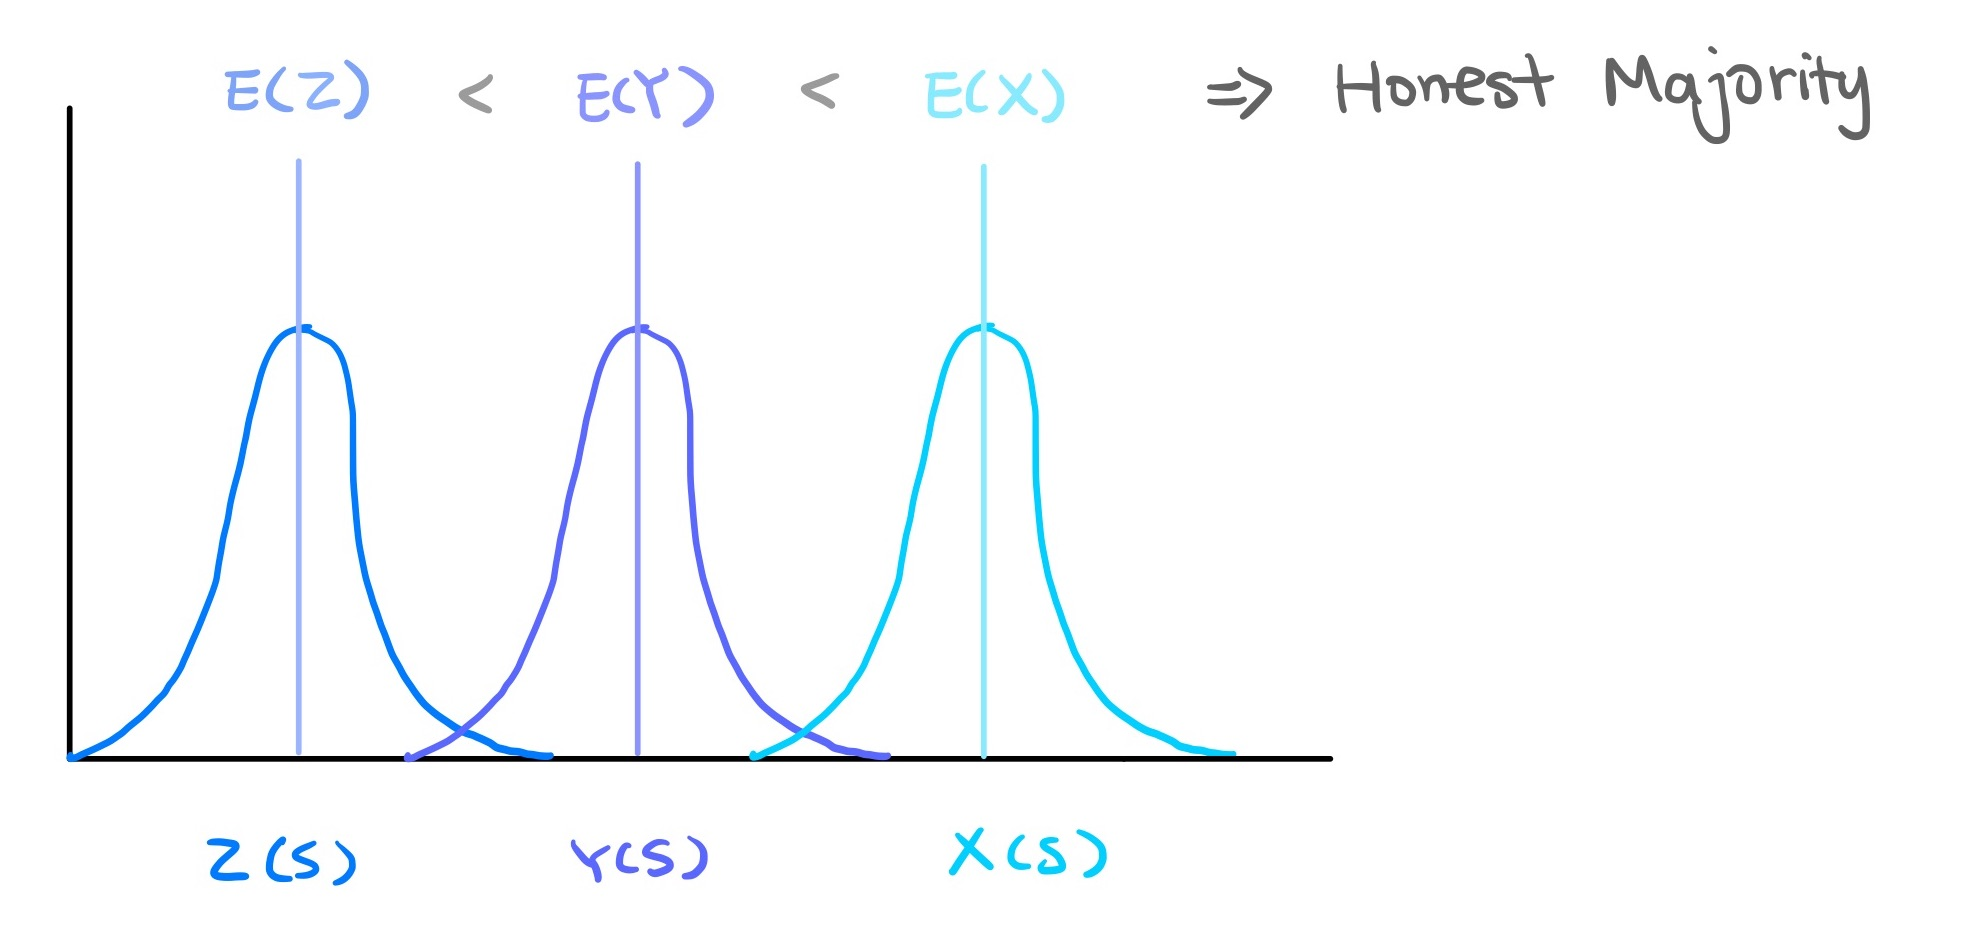
\includegraphics[width=14cm]{figures/honest-maj}
    \caption{Illustration of the probability density functions for $X(S)$, $Y(S)$, and $Z(S)$. Note that $\E[Z(S)] < \E[Y(S)] < \E[X(S)]$}
    \label{fig:expectation_gap}
\end{figure}

But if we want common prefix to hold except with negligible probability, it is not sufficient that the \emph{expectations} are in this order. It is not sufficient that \emph{on average} the adversary will have fewer successful queries than the honest parties will have convergence opportunities. We want something stronger: except with negligible probability, in all large enough intervals of consecutive slots $S$, the adversary will have fewer successful queries than the honest parties will have convergence opportunities, i.e. $\Pr[\forall S\colon Z(S) < Y(S)] \geq 1 - \negl(\kappa)$. In other words, the expectations of $X(S)$, $Y(S)$, and $Z(S)$ must be sufficiently separated so that the probability of $Y(S) \leq Z(S)$ is negligible.

In order to prove $\Pr[Y(S) < Z(S)] = \negl(\kappa)$, we will use a probability tool called the Chernoff Bound and introduce the concept of \textit{typicality}.

\subsubsection{Chernoff Bound}

We will not prove this theorem here, but intuitively, the Chernoff Bound says this: if we flip a fair coin $n$ times, where heads = 1 and tails = 0, then the more tosses we have, the less likely their sum is going to deviate from the expected value of their sum, which is $0.5 \times n$. As the number of trials increases, the probability that the sum is off the expectation by a certain \emph{percentage} of error approaches 0 (this probability is represented by the shaded regions in Figure~\ref{fig:balancing_eq}). More formally, the Chernoff Bound states:

\begin{theorem}
Consider random variables ${X_i}$, ${i\in [n]}$ s.t. $X_i \overset{\text{i.i.d.}}{\sim} \mathrm{Bernoulli}(p)$ and $X = \sum_{i=1}^{n} X_i$. For any $\epsilon > 0$,
\begin{align}
    \Pr[X \leq (1 - \epsilon) \mu ] &\leq e^{-\Omega(n\epsilon^2\mu)}, \\
    \Pr[X \geq (1 + \epsilon) \mu ] &\leq e^{-\Omega(n\epsilon^2\mu)}.
\end{align}
\end{theorem}
For more details about the Chernoff bound and its proof, a good reference is \cite{chernoff}.
(This $\mu$ is internal to the Chernoff bound and is not the chain quality parameter.)


\subsubsection{Typicality}

Ultimately, we want to prove that common prefix and chain growth are satisfied except with negligible probability. In order to simplify our analysis of probabilities, we introduce the concept of ``typicality''. Typical executions will be defined such that executions will be typical except with negligible probability. If we show that typical executions uphold chain growth and common prefix, then we will have proven that chain growth and common prefix hold except with negligible probability.

\begin{definition}[$(\epsilon,\lambda)$-Typical executions]
An execution is typical if for all sets of consecutive rounds $S$ with $|S| \geq \lambda$:
\begin{enumerate}
    \item $(1-\epsilon) E[X(S)] < X(S) < (1+\epsilon) E[X(S)]$
    \item $(1-\epsilon) E[Y(S)] < Y(S) $
    \item $ Z(S) < E[Z(S)] + \epsilon E[X(S)] $
\end{enumerate}
In addition, there are no collisions or predictions in the Random Oracle.
\end{definition}

\begin{theorem}
$(\epsilon,\lambda)$-Typical executions occur with probability at least $1-\negl(\lambda)$.
\end{theorem}

\begin{proof} We can show that each of the three properties hold with $(1-\negl(\lambda))$ probability, where $n=|S| \geq \lambda$.

\begin{enumerate}
    \item Directly by Chernoff bound, this is true with probability $\geq 1 - e^{-\Omega(n\epsilon^2)}$.

    \item By the left-sided Chernoff bound, we have that $(1-\epsilon) E[Y(S)] < Y(S) $ is true with probability $\geq 1 - e^{-\Omega(n\epsilon^2)}$.
    % We also know $X(S) \leq Y(S)$ with probability 1 because convergence opportunity rounds are a subset of rounds where at least one honest block is mined. Connecting the two inequalities we have $(1-\epsilon) E[X(S)] < X(S) \leq Y(S)$, so $(1-\epsilon) E[X(S)] < Y(S)$.

    \item By the right-sided Chernoff bound, we have that $ Z(S) < (1+\epsilon) E[Z(S)] = E[Z(S)] + \epsilon E[Z(S)] $ is true with probability $\geq 1 - e^{-\Omega(n\epsilon^2)}$. By the honest majority assumption, we expect $E[Z(S)] < E[X(S)]$ because less computing power implies fewer expected successful queries (this will be proven momentarily). Since $\epsilon$ is positive, $\epsilon E[Z(S)] < \epsilon E[X(S)]$. All together we have $ Z(S) < (1+\epsilon) E[Z(S)] = E[Z(S)] + \epsilon E[Z(S)] < E[Z(S)] + \epsilon E[X(S)]$.

    \item Since the Random Oracle randomly samples each output from $\{0,1\}^{\kappa}$, the probability that it samples the same output for two different inputs is $\negl(\kappa)$. Similarly, the probability that the adversary can predict the output for an input it has not queried before is $\negl(\kappa)$. The probability that a collision or prediction occurs over a polynomial time execution is also $\negl(\kappa)$. (We will choose $\kappa = \Omega(\lambda)$).
\end{enumerate}

Note that the reason we can use the Chernoff Bound is because we are using the random oracle model, which gives us that each query to the random oracle being successful is an independent Bernoulli random variable, hence the random sequences $X, Y$, and $Z$ are independent across time ($X_r$ and $Y_r$ are not independent, but $X_r$ and $X_{r'}$ for $r \neq r'$ are). This is stronger than just a collision-resistant hash function.

\end{proof}

Note that we need the set $S$ to be of size at least $\lambda$ to allow the variables to be concentrated within a Chernoff error $\epsilon$, because Chernoff bound requires a large enough number of trials to be invoked.

For reasons that we will see soon, we will choose $\epsilon$ and $f$ so that $3f + 3\epsilon \leq \delta$. This is called the \emph{balancing equation}. Here, $\delta$ is the honest advantage, i.e., $t < (1-\delta)(n-t)$.

Now remember our goal is to prove that the expectations of $X$, $Y$, and $Z$ must be sufficiently separated so that $Y(S) > Z(S)$ except with negligible probability, i.e. we want to show that the lower bound of $Y(S)$ is larger than the upper bound of $Z(S)$. Typicality gives us bounds on $X(S), Y(S), Z(S)$ but they are with respect to $\E[X(S)], \E[Y(S)], \E[Z(S)]$, so we need to find bounds for these expectations respectively.
Since the random variables $X_r$ are independent and identically distributed for different $r$, $\E[X(S)] = |S|\E[X_r]$. Similarly, $\E[Y(S)] = |S|\E[Y_r]$ and $\E[Z(S)] = |S|\E[Z_r]$. So, we only need to compare $\E[X_r]$, $\E[Y_r]$ and $\E[Z_r]$.

What do we know about $\E[X_r]$?
\begin{align}
    \E[X_r] = f &= \Pr [\text{at least one successful honest query in round $r$}] \nonumber \\
    & = 1 - \Pr [\text{no honest query succeeds in round $r$}] \nonumber \\
    & = 1 - (1-p)^{q(n-t)} \nonumber \\
    & < pq(n-t).
\end{align}

The last step above comes from Bernoulli's inequality, i.e,  $(1+x)^a > 1+ax, \forall x, a \in \mathbb{R}, x > -1, x \neq 0, a > 1$. We can also show that
\begin{align}
\label{eq:f_lower_bound}
    \frac{f}{1-f} = \frac{1-(1-p)^{q(n-t)}}{(1-p)^{q(n-t)}} = (1-p)^{-q(n-t)} -1 > (1+p)^{q(n-t)} - 1 > pq(n-t).
\end{align}
Therefore, we can sandwich the value of $\E[X_r]$ by its lower and upper bounds.
\begin{align}
    (1-f)pq(n-t) < \E[X_r] < pq(n-t).
\end{align}

% This is a bound on $\E[X]$ which is always true (not just with $\negl(\kappa)$ probability).\\

For $\E[Y_r]$, we have
\begin{align}
\label{eq:y_lower_bound}
    \E[Y_r]  \geq q(n-t)p (1-p)^{q(n-t)-1} > pq(n-t)[1-pq(n-t)] \geq f (1-f).
\end{align}
The first inequality is obtained by assuming that all honest parties make all $q$ queries even after a successful one and summing over all queries the probability $p(1-p)^{q(n-t)-1}$ that it is the only successful one.
The second inequality uses $(1-p)^{q(n-t)-1} > (1-p)^{q(n-t)}$ and uses Bernoulli's inequality again.
The third inequality holds because $f(1-f)$ is an increasing function for $f \in (0,\frac12)$.

Since the adversary is allowed at most $qt$ queries in each round and each query is successful with probability $p$, we also have
\begin{align}
    \E[Z_r] = pqt.
\end{align}

Even though we want the expectations of $X(S)$, $Y(S)$, and $Z(S)$ to be sufficiently separated so that $Y(S) > Z(S)$ except with negligible probability, we cannot separate them arbitrarily far. This is because the distance between $\E[Z]$ and $\E[X]$ is determined by the advantage held by the majority in the honest majority assumption, i.e., $t \leq (1-\delta)(n-t)$ where $3f+3\epsilon \leq \delta$.
To see this,
\begin{align}
    \E[Z_r] = pqt = \frac{t}{n-t} \cdot pq(n-t) < \frac{t}{n-t} \cdot \frac{f}{1-f} < \left(1+\frac{\delta}{2}\right)\cdot f \cdot \frac{t}{n-t}.
\end{align}
Here, we have used the inequality $\frac{f}{1-f} > pq(n-t)$ proved in \eqref{f_lower_bound}, and another inequality $\frac{1}{1-f} < 1 + \frac{\delta}{2}$. To prove the second inequality, we know that $f < \frac{\delta}{3}$ because $3f+3\epsilon \leq \delta$ and $\epsilon>0$. So, we need to show that $\frac{1}{1-\delta/3} < 1+\frac{\delta}{2}$ which can be verified as follows:
\begin{align*}
    1 &< \left(1-\frac{\delta}{3}\right) \left(1+\frac{\delta}{2}\right) \\
    \iff 1 &< 1 + \frac{\delta}{2} - \frac{\delta}{3} - \frac{\delta^2}{6} \\
    \iff 0 &< \frac{\delta}{6} - \frac{\delta^2}{6} \\
    \iff 0 &< \frac{\delta}{6}(1-\delta)
\end{align*}
which is true because $0 < \delta < 1$.

The honest advantage $\delta$ (which is the distance between $|S|pqt$ and $|S|pq(n-t)$, scaled by $|S|pq(n-t)$) is composed of the distance between $\E[Z(S)]=|S|pqt$ and $\E[Y(S)]$, distance between $\E[Y(S)]$ and $\E[X(S)]$, and distance between $\E[X(S)]$ and $|S|pq(n-t)$. We allocate this total possible distance by following balancing equation: $3\epsilon + 3f \leq \delta$. Let's break this inequality down for an intuitive understanding along with Figure~\ref{fig:balancing_eq}.

\begin{itemize}
    \item $3 \epsilon$ is the relative distance we allocate between $\E[Z(S)]$ and $\E[Y(S)]$, where $\epsilon$ is the Chernoff error. By Chernoff, we have that $Z(S)$ should not exceed $(1+\epsilon)\E[Z(S)]$ with more than negligible probability, and likewise $Y(S)$ should not go below $(1-\epsilon)\E[Y(S)]$. Therefore, if we leave some buffer distance between $(1+\epsilon)\E[Z(S)]$ and $(1-\epsilon)\E[Y(S)]$ we should have that $Y(S) > Z(S)$ except with negligible probability. So we secure $\epsilon$ to the right of $\E[Z(S)]$, $\epsilon$ to the left of $\E[Y(S)]$, and another $\epsilon$ in between as a buffer, which gives us $3 \epsilon$.

    \item The probability of an honestly successful round is $f=\E[X_r]$. Recall that we have calculated that $\E[Y_r] \geq f (1-f)$ in \eqref{y_lower_bound}, so $\E[Y(S)]$ is at most $f$ relative distance away from $\E[X(S)]$. Following similar logic as above, we secure $f$ to the right of $\E[Y(S)]$ and $f$ to the left of $\E[X(S)]$.

    \item Finally, $\E[X(S)]$ is at most $f$ relative distance away from $|S|pq(n-t)$. We get this from \eqref{f_lower_bound}.

    % \item $\delta$ is the honest advantage, i.e. the difference between $\E[X]$ and $\E[Z]$ from $\E[X] - \E[Z] \geq \delta \E[X]$ as discussed above.
\end{itemize}

Note the relationship between $\lambda$ and $\epsilon$. The smaller we require our Chernoff error $\epsilon$ to be, the longer time $\lambda$ we need to wait for this concentration to occur. If we look at the Chernoff bound equations, the probability that our variables \emph{fail} to be nicely concentrated is approximately $e^{-\Omega(\epsilon^2 \lambda f)}$ (since the expectations of $X(S)$, $Y(S)$, $Z(S)$ are proportional to $\lambda f$). Recall from the previous lectures that we denoted by $\kappa$ our security parameter, and this indicated the \emph{bits} in our accepted probability of \emph{failure}. Our accepted probability of failure was then at most in the order of $2^{-\kappa}$. We want to achieve the same thing with our choice of $\epsilon$ and $\lambda$. Therefore, given a particular $\kappa$ (for example $\kappa = 256$) and particular values for $\epsilon$ and $f$, we need to set $\lambda$ such that $\kappa \approx \epsilon^2 \lambda f$. In a nutshell, the larger we make $\epsilon$, the less time $\lambda$ we will need to wait for confirmation.

So, we want both  $\epsilon$ to be large (to achieve fast confirmation and a small $\lambda$), but also $f$ to be large (to achieve good chain growth with a fast block production rate). However, we cannot make both of them arbitrarily large, as they have to satisfy the balancing equation: $3f + 3\epsilon \leq \delta$. The value $\delta$ is not a parameter we can change, but is given to us from the threat model and adversarial assumptions: It is telling us what sort of adversary we are able to withstand. In the end, for a given $\delta$, we want to have the fastest possible blockchain, yet maintain security. Splitting equally between $\epsilon$ and $f$, we can choose $\epsilon = f = \delta/6$. The takehome lesson is that, to withstand a powerful adversary (small $\delta$), we need to wait a sufficient amount of time for transactions to be confirmed. You cannot have both quick confirmation and good security!

In the next chapter, we will use the tools developed today to show that in typical executions, $Y(S) > Z(S)$ for all intervals of slots $S$ with $|S|\geq \lambda$. This will help us to prove that Common Prefix and Chain Growth hold in typical executions.

\begin{landscape}\centering
\begin{figure*}
    \centering
    \vspace*{\fill}
    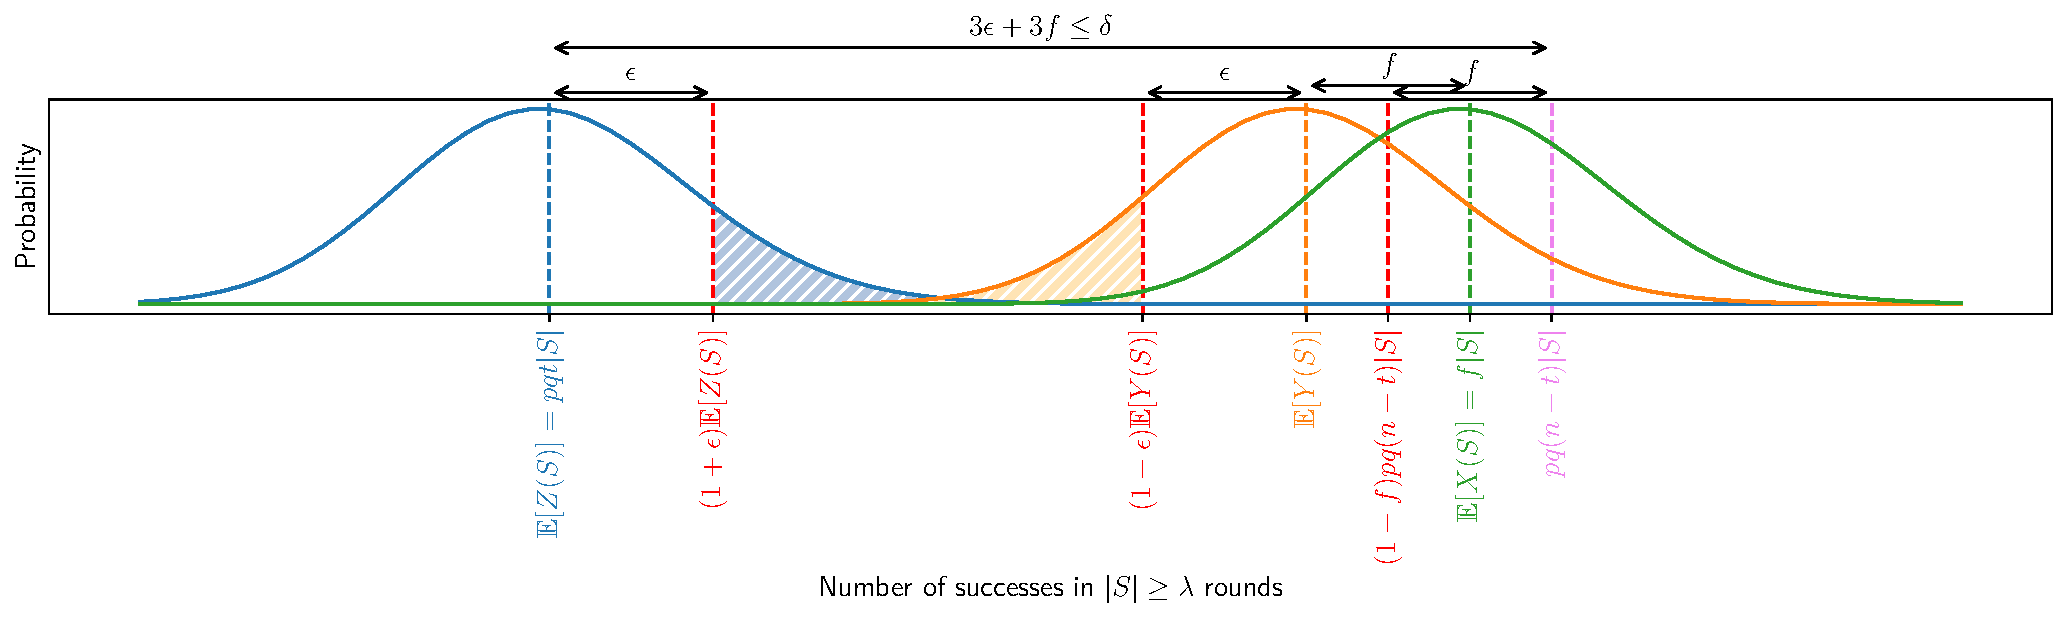
\includegraphics[width=\linewidth]{figures/backbone-vars.pdf}
    \caption{The distribution of the random variables $X$, $Y$, and $Z$ in the proof-of-work longest chain protocol.}
    \label{fig:balancing_eq}
    \vspace*{\fill}
\end{figure*}
\end{landscape}

